\begin{myexem}
  \label{exem:run4}
  We tried the atom extraction procedure and Algorithm~\ref{algo:prodl} for $l = 1$ and $l = 3$ on our running example;
  see Example~\ref{exem:run1}, Example~\ref{exem:run2} and Example~\ref{exem:run3}.
  The code used to obtain the results of this example can be found on the author's website. %
  The result is shown in \figref{pedj}.
  We showed in \cite{legat2016generating} that the CJSR of the system is equal to 0.97482.
  We can see that this lower bound is found for $d = 4$ for $l=1$ and for $d=1$ for $l=3$.
  The atom extraction finds the lower bound 0.939255.
\end{myexem}

\begin{figure}[!ht]
  \begin{subfigure}{0.48\textwidth}
    \centering
    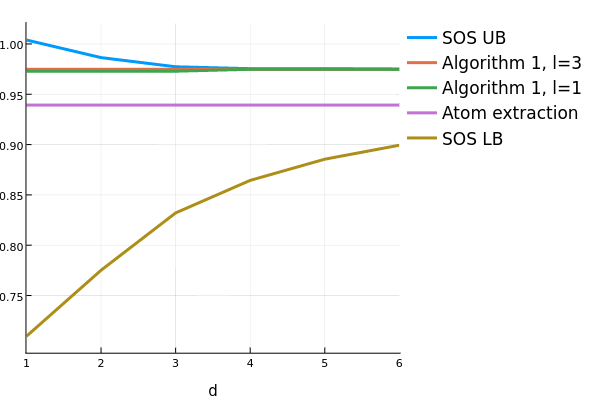
\includegraphics[width=\textwidth]{../../latex/images/PEDJ.png}
  \end{subfigure}
  \begin{subfigure}{0.48\textwidth}
    \centering
    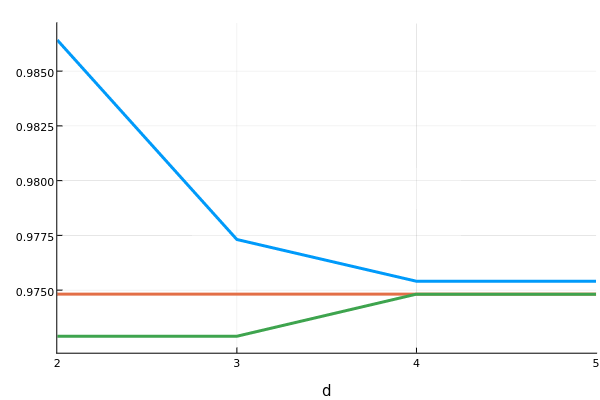
\includegraphics[width=\textwidth]{../../latex/images/PEDJ_zoom.png}
  \end{subfigure}
  \caption{Result of \exemref{run4}. The SOS UB is the upper bound found by \progref{primal} and the SOS LB is obtained from this upper bound the guarantee given in \cororef{mix}. The value $d$ of horizontal axis corresponds to using polynomials of degree $2d$. The right figure is a zoom of the left figure.}
  \label{fig:pedj}
\end{figure}
